\newcommand{\installerTagResultsAucTable}{
    \begin{table}[H]
        \centering
        \begin{tabular}{|p{2,8cm}||P{2,2cm} P{2,2cm} P{2,2cm} P{2,2cm}|}
            \hline
            Installer Tag & ALOHA\newline (M/B only) & ALOHA & Joint\newline Embedding & Proposed\newline Model \\
            \hline
            AUC-ROC & - & 0.967$\pm$0.007 & \textBF{0.975$\pm$0.001} & \textBF{0.975$\pm$0.001} \\
            \hline
        \end{tabular}
        \caption[Installer Tag prediction task AUC-ROC results]{AUC-ROC (Area Under Curve) of the different models for the \textbf{Installer Tag} prediction task. Results were aggregated over \textBF{3} training runs with different weight initializations and minibatch orderings. Best results are shown in \textbf{bold}.} \label{tab:installerTag_auc}
    \end{table}
}

\newcommand{\installerTagResultsAtFprTable}{
    \begin{center}
        \begin{longtable}[c]{|P{3,2cm}||P{1,8cm} P{1,8cm} P{1,8cm} P{1,8cm} P{1,8cm}|}
            \hline
            Installer Tag & \multicolumn{5}{c|}{{FPR}} \\
            & $10^{-5}$ & $10^{-4}$ & $10^{-3}$ & $10^{-2}$ & $10^{-1}$ \\
            \hline
            \endfirsthead

            \caption*{\raggedright ...continued from previous page} \\
            \hline
            Installer Tag & \multicolumn{5}{c|}{\textbf{FPR}} \\
            & $10^{-5}$ & $10^{-4}$ & $10^{-3}$ & $10^{-2}$ & $10^{-1}$ \\
            \hline
            \endhead

            \caption*{\raggedleft ...continued on next page} \\
            \endfoot

            \caption[Installer Tag prediction task results]{Mean and standard deviation results (TPR, Accuracy, Recall, Precision and F1-Score) of the different models for the \textbf{Installer Tag} prediction task at different \textbf{FPR}s (\textit{False Positive Rates}). Results were aggregated over \textBF{3} training runs with different weight initializations and minibatch orderings. Best results are shown in \textbf{bold}. Under \textbf{TPR} results are also presented the percentage reduction in mean detection error and in ROC curve standard deviation introduced by the \textit{Proposed Model} with respect to both \textit{ALOHA} model and \textit{Joint Embedding}.} \label{tab:installerTag_results_at_fpr} \\
            \endlastfoot

            \multicolumn{6}{|c|}{\textbf{TPR}} \\
            \hline
            ALOHA (M/B only) & - & - & - & - & - \\
            ALOHA & 0.106$\pm$0.073 & 0.206$\pm$0.011 & 0.388$\pm$0.059 & 0.717$\pm$0.054 & 0.927$\pm$0.021 \\
            Joint Embedding & 0.191$\pm$0.013 & 0.292$\pm$0.026 & 0.506$\pm$0.054 & \textBF{0.777$\pm$0.010} & \textBF{0.944$\pm$0.006} \\
            Proposed Model & \textBF{0.208$\pm$0.009} & \textBF{0.343$\pm$0.033} & \textBF{0.527$\pm$0.063} & 0.759$\pm$0.042 & 0.926$\pm$0.013 \\
            \hline
            Error Reduction wrt\newline ALOHA (M/B only) & - & - & - & - & - \\
            Error Reduction wrt\newline ALOHA & 11.4\% & 17.3\% & 22.7\% & 14.8\% & -1.4\% \\
            Error Reduction wrt\newline Joint Embedding & 2.1\% & 7.2\% & 4.3\% & -8.1\% & -32.1\% \\
            \hline
            Std Reduction wrt\newline ALOHA (M/B only) & - & - & - & - & - \\
            Std Reduction wrt\newline ALOHA & 87.7\% & -200.0\% & -6.8\% & 22.2\% & 38.1\% \\
            Std Reduction wrt\newline Joint Embedding & 30.8\% & -26.9\% & -16.7\% & -320.0\% & -116.7\% \\
            \hline
            \multicolumn{6}{|c|}{\textbf{Accuracy}} \\
            \hline
            ALOHA (M/B only) & - & - & - & - & - \\
            ALOHA & 0.984$\pm$0.001 & 0.986$\pm$0.000 & 0.988$\pm$0.001 & 0.985$\pm$0.001 & 0.900$\pm$0.000 \\
            Joint Embedding & \textBF{0.986$\pm$0.000} & 0.987$\pm$0.000 & 0.990$\pm$0.001 & \textBF{0.986$\pm$0.000} & \textBF{0.901$\pm$0.000} \\
            Proposed Model & \textBF{0.986$\pm$0.000} & \textBF{0.988$\pm$0.001} & \textBF{0.991$\pm$0.001} & 0.986$\pm$0.001 & 0.900$\pm$0.000 \\
            \hline
            \multicolumn{6}{|c|}{\textbf{Recall}} \\
            \hline
            ALOHA (M/B only) & - & - & - & - & - \\
            ALOHA & 0.106$\pm$0.073 & 0.206$\pm$0.011 & 0.388$\pm$0.059 & 0.717$\pm$0.054 & 0.927$\pm$0.021 \\
            Joint Embedding & 0.191$\pm$0.013 & 0.292$\pm$0.026 & 0.506$\pm$0.054 & \textBF{0.777$\pm$0.010} & \textBF{0.944$\pm$0.006} \\
            Proposed Model & \textBF{0.208$\pm$0.009} & \textBF{0.343$\pm$0.033} & \textBF{0.527$\pm$0.063} & 0.759$\pm$0.042 & 0.926$\pm$0.013 \\
            \hline
            \multicolumn{6}{|c|}{\textbf{Precision}} \\
            \hline
            ALOHA (M/B only) & - & - & - & - & - \\
            ALOHA & 0.955$\pm$0.059 & 0.974$\pm$0.001 & 0.873$\pm$0.017 & 0.564$\pm$0.019 & 0.144$\pm$0.003 \\
            Joint Embedding & \textBF{0.997$\pm$0.000} & 0.981$\pm$0.002 & 0.901$\pm$0.010 & \textBF{0.584$\pm$0.003} & \textBF{0.146$\pm$0.001} \\
            Proposed Model & \textBF{0.997$\pm$0.000} & \textBF{0.984$\pm$0.001} & \textBF{0.904$\pm$0.011} & 0.578$\pm$0.014 & 0.144$\pm$0.002 \\
            \hline
            \multicolumn{6}{|c|}{\textbf{F1 Score}} \\
            \hline
            ALOHA (M/B only) & - & - & - & - & - \\
            ALOHA & 0.184$\pm$0.126 & 0.340$\pm$0.015 & 0.535$\pm$0.060 & 0.631$\pm$0.033 & 0.249$\pm$0.005 \\
            Joint Embedding & 0.321$\pm$0.018 & 0.449$\pm$0.032 & 0.646$\pm$0.048 & \textBF{0.667$\pm$0.005} & \textBF{0.253$\pm$0.001} \\
            Proposed Model & \textBF{0.345$\pm$0.012} & \textBF{0.507$\pm$0.036} & \textBF{0.664$\pm$0.054} & 0.656$\pm$0.024 & 0.249$\pm$0.003 \\
            \hline
        \end{longtable}
    \end{center}
}

\newcommand{\installerTagResultsSummaryTable}{
    \begin{table}[H]
        \centering
        \begin{tabular}{|P{3,2cm}||P{1,8cm} P{1,8cm} P{1,8cm} P{1,8cm} P{1,8cm}|}
            \hline
            \multicolumn{6}{|c|}{Installer Tag (at FPR $=1\%$)} \\
            \hline
            Model & TPR & Accuracy & Precision & Recall & F1 score \\
            \hline
            ALOHA (M/B only) & - & - & - & - & - \\
            ALOHA & 0.717$\pm$0.054 & 0.985$\pm$0.001 & 0.564$\pm$0.019 & 0.717$\pm$0.054 & 0.631$\pm$0.033 \\
            Joint Embedding & \textBF{0.777$\pm$0.010} & \textBF{0.986$\pm$0.000} & \textBF{0.584$\pm$0.003} & \textBF{0.777$\pm$0.010} & \textBF{0.667$\pm$0.005} \\
            Proposed Model & 0.759$\pm$0.042 & 0.986$\pm$0.001 & 0.578$\pm$0.014 & 0.759$\pm$0.042 & 0.656$\pm$0.024 \\
            \hline
        \end{tabular}
        \caption[Summary of Installer Tag prediction task results]{Summary of the mean and standard deviation results of the different models for the \textbf{Installer Tag} prediction task at \textbf{FPR} $=1\%$. Results were aggregated over \textBF{3} training runs with different weight initializations and minibatch orderings. Best results are shown in \textbf{bold}.} \label{tab:installerTag_result_summary}
    \end{table}
}

\newcommand{\installerTagRocAlohaMB}{
    \begin{figure}[H]
        \vspace*{-0.5cm}
        \centering
        \includegraphics[width=0.6\textwidth]{./results/installer_tag_roc_alohaMB.png}
        \vspace*{-0.2cm}
        \caption[Installer Tag prediction task ALOHA (M/B only) ROC curve]{ROC curve and AUC statistics of \textBF{ALOHA (M/B only)} model for the \textbf{Installer Tag}. The line represents the \textit{mean} TPR at a given FPR, while the shaded region represents the \textit{standard deviation}. Statistics were computed over \textBF{3} training runs, each with random parameter initialization.}
        \label{fig:installerTagRocAlohaMB}
    \end{figure}
}

\newcommand{\installerTagRocAloha}{
    \begin{figure}[H]
        \vspace*{-0.5cm}
        \centering
        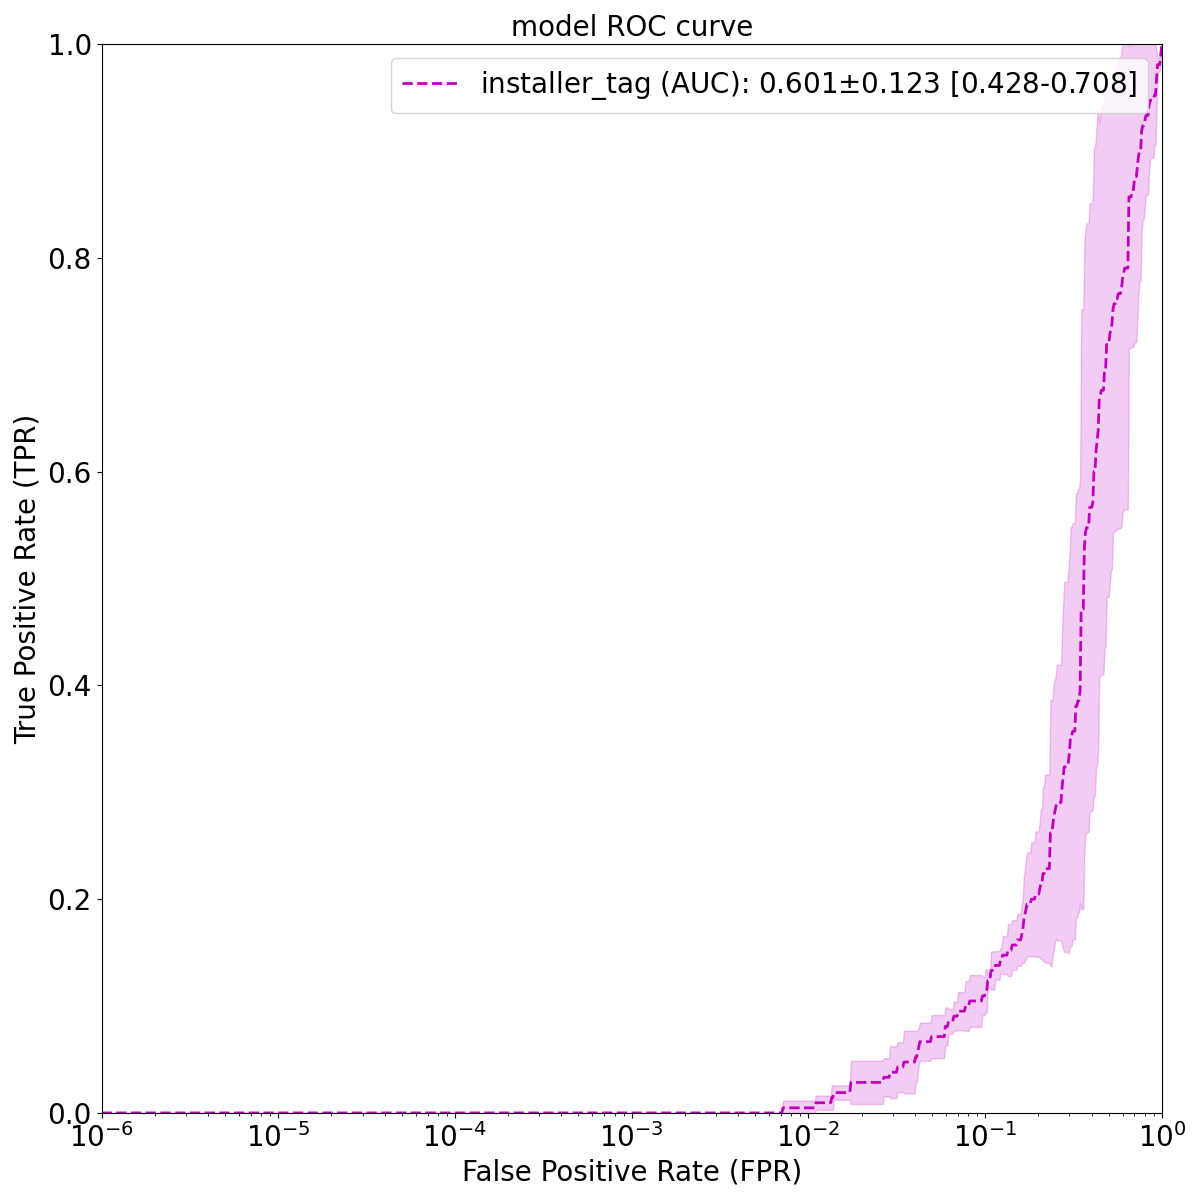
\includegraphics[width=0.6\textwidth]{./results/installer_tag_roc_aloha.png}
        \vspace*{-0.2cm}
        \caption[Installer Tag prediction task ALOHA ROC curve]{ROC curve and AUC statistics of \textBF{ALOHA} model for the \textbf{Installer Tag}. The line represents the \textit{mean} TPR at a given FPR, while the shaded region represents the \textit{standard deviation}. Statistics were computed over \textBF{3} training runs, each with random parameter initialization.}
        \label{fig:installerTagRocAloha}
    \end{figure}
}

\newcommand{\installerTagRocJointEmbedding}{
    \begin{figure}[H]
        \vspace*{-0.5cm}
        \centering
        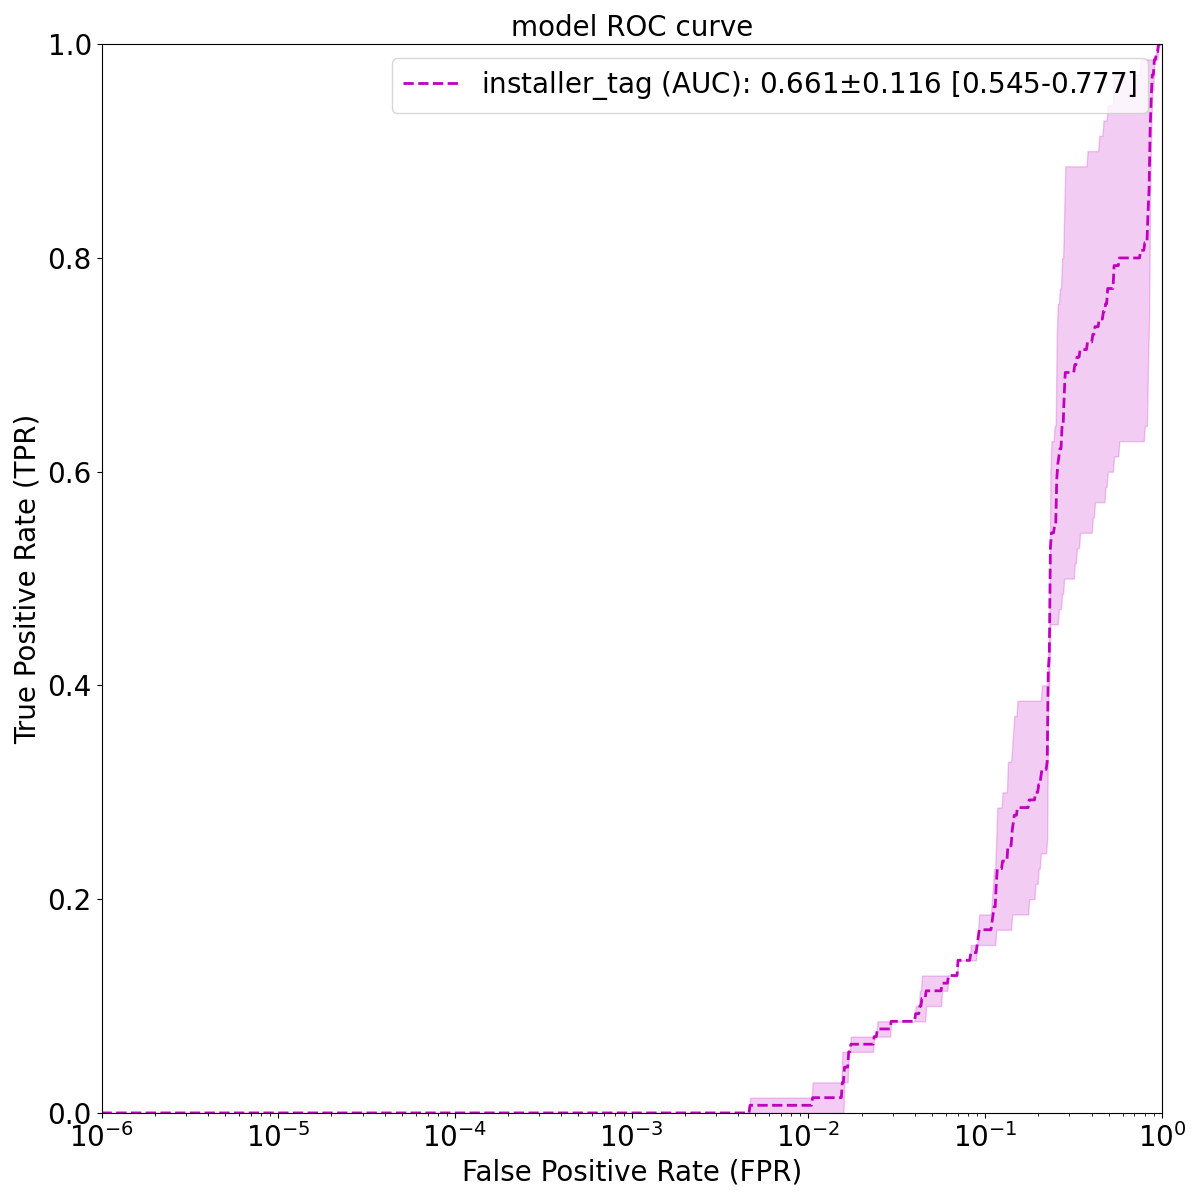
\includegraphics[width=0.6\textwidth]{./results/installer_tag_roc_jointEmbedding.png}
        \vspace*{-0.2cm}
        \caption[Installer Tag prediction task Joint Embedding ROC curve]{ROC curve and AUC statistics of \textBF{Joint Embedding} model for the \textbf{Installer Tag}. The line represents the \textit{mean} TPR at a given FPR, while the shaded region represents the \textit{standard deviation}. Statistics were computed over \textBF{3} training runs, each with random parameter initialization.}
        \label{fig:installerTagRocJointEmbedding}
    \end{figure}
}

\newcommand{\installerTagRocProposedMethod}{
    \begin{figure}[H]
        \vspace*{-0.5cm}
        \centering
        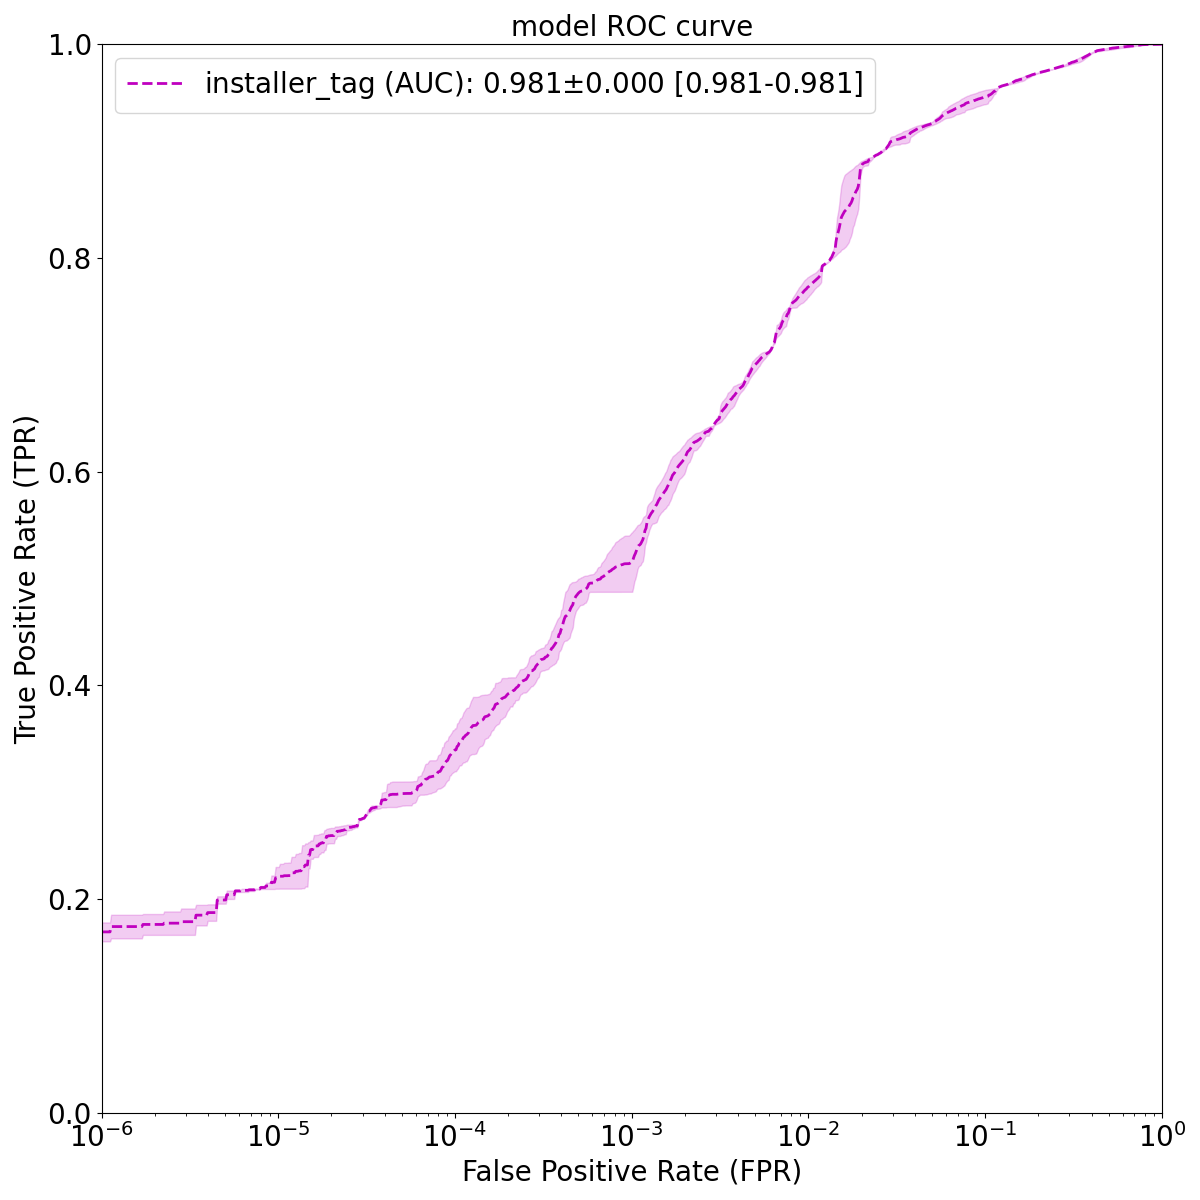
\includegraphics[width=0.6\textwidth]{./results/installer_tag_roc_proposedModel.png}
        \vspace*{-0.2cm}
        \caption[Installer Tag prediction task Proposed Model ROC curve]{ROC curve and AUC statistics of \textBF{Proposed Model} for the \textbf{Installer Tag}. The line represents the \textit{mean} TPR at a given FPR, while the shaded region represents the \textit{standard deviation}. Statistics were computed over \textBF{3} training runs, each with random parameter initialization.}
        \label{fig:installerTagRocProposedModel}
    \end{figure}
}
